\chapter{绪论}
\section{研究背景}
分层存储系统(Tiered Storage System),又称为层级存储管理(Hierarchical Storage Management),是当前各领域存储系统的主流架构。其基本特点是将文件数据存储在若干层级的存储介质中,不同层级的介质(DRAM,SSD,HDD等)具有不同的容量、吞吐率、访问延迟与成本等。不同的应用负载和场景下,存储系统中的数据重要性存在差异,可以粗略地分为“热”数据与“冷”数据:正在访问与频繁访问的“热”数据优先存储于更接近CPU、访问更快的内存、SSD阵列等存储介质中;近期没有访问需求或访问频率低的“冷”数据主要存储在低层级的磁盘阵列或远程存储服务器中。在现实应用中,数据的“热”与“冷”不是静态的,而是随着应用的访问需求动态变化,数据在不同层级之间的迁移管理成为层次存储系统的基本任务之一。
\begin{figure}[htp]
    \centering
    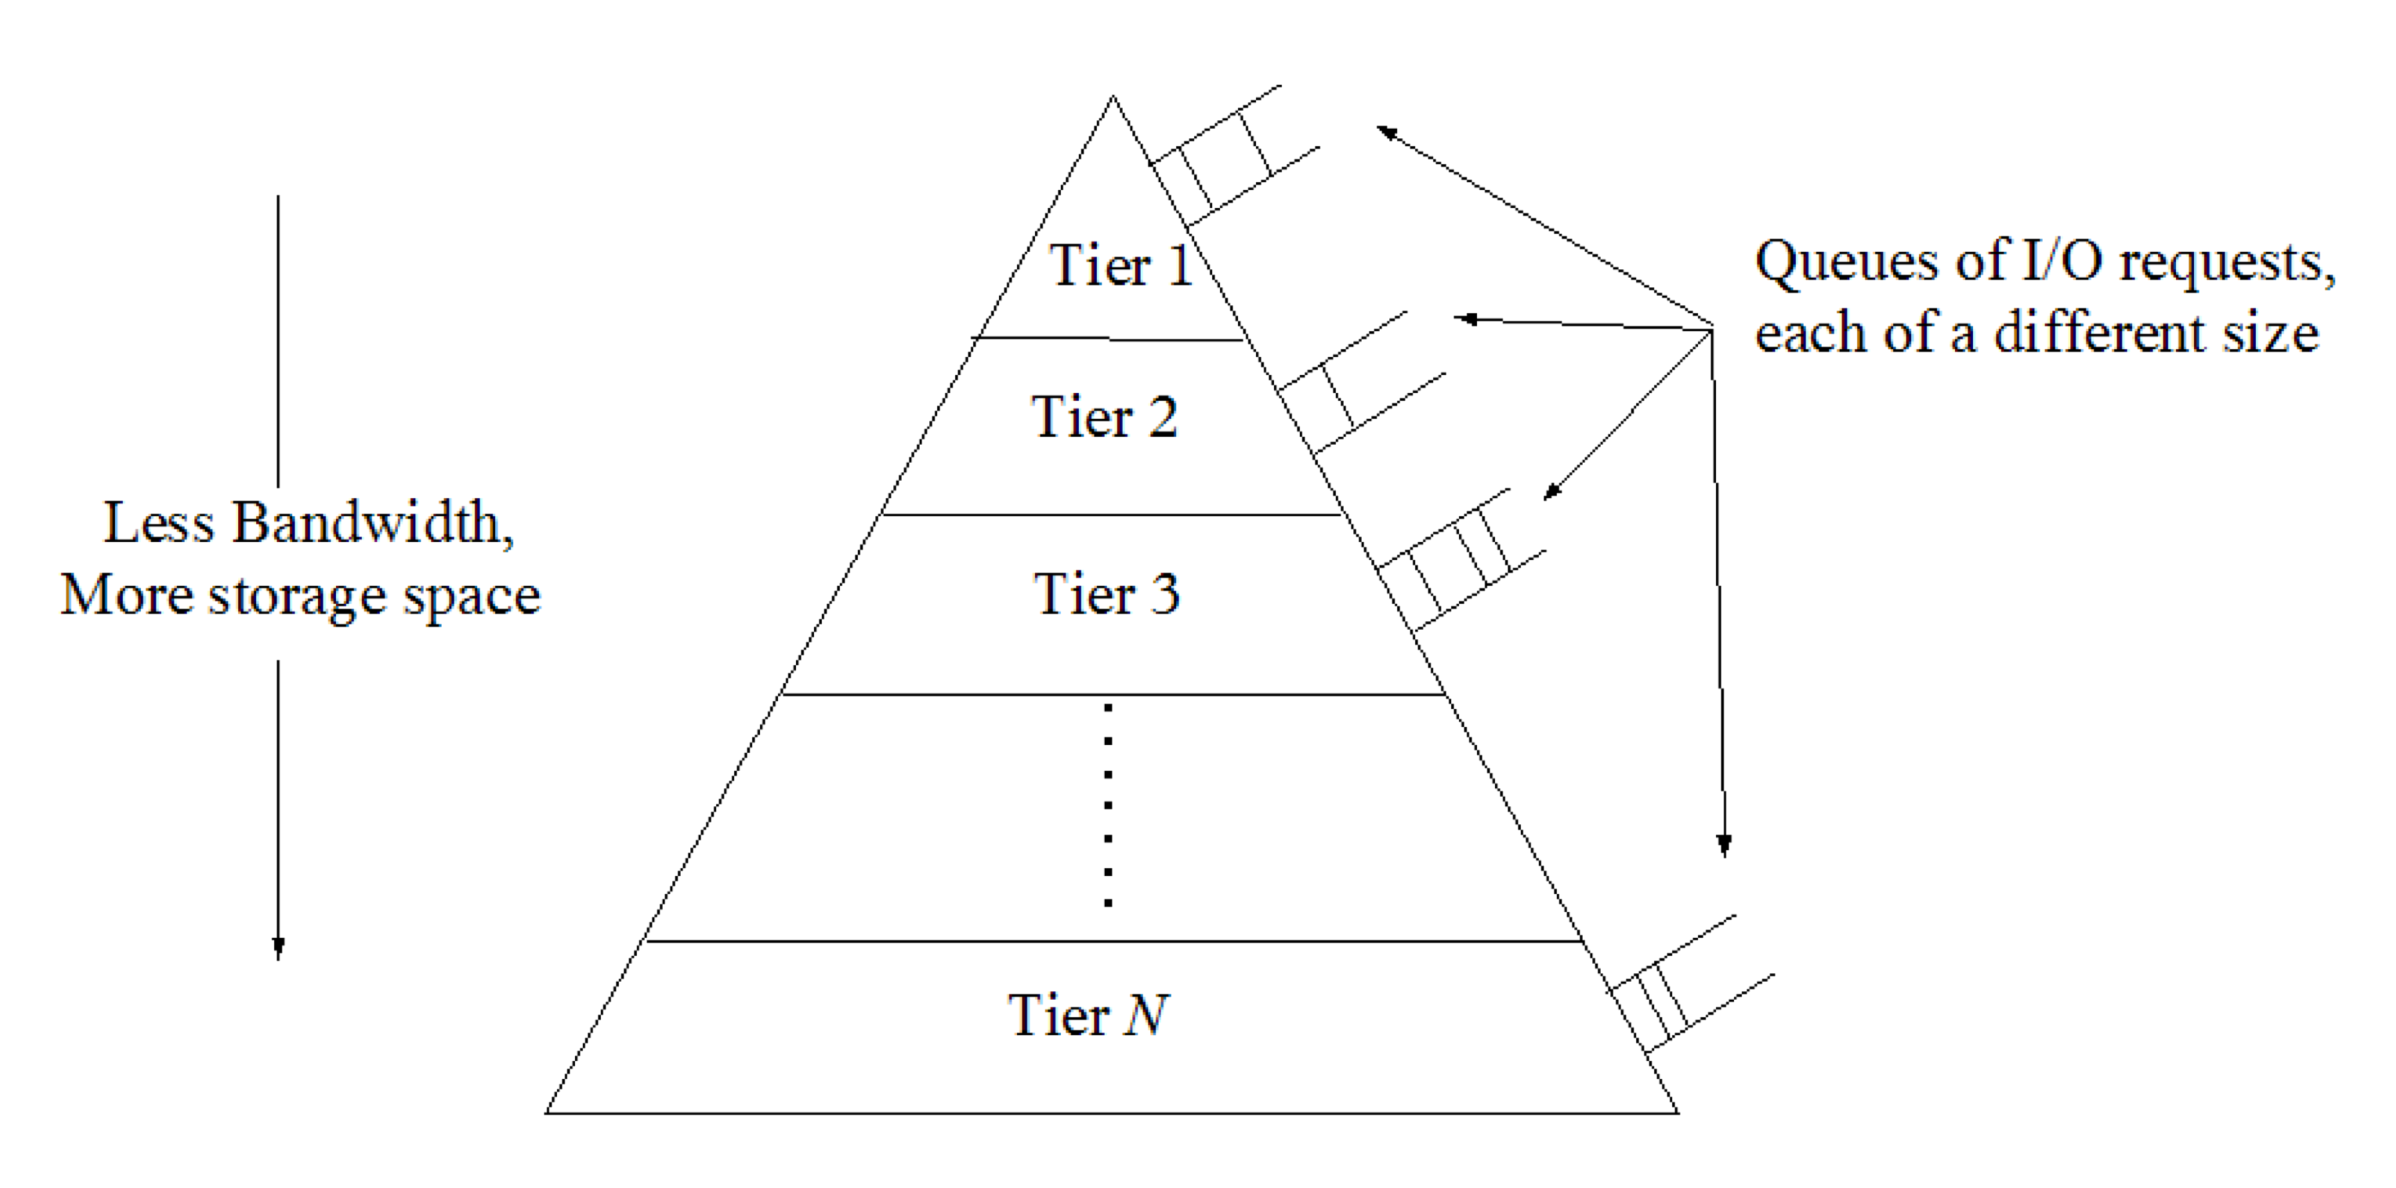
\includegraphics[width=\textwidth]{chp2_multi_tiers}
    \caption{分层存储系统(Tiered Storage System)}
    \label{fig:multi_tiers}
\end{figure}
如图\ref{fig:multi_tiers}所示,分层存储系统按层级从高到低由不同存储介质组成:
高层级存储通常由内存DRAM(Dynamic Random Access Memory)、非易失性存储(Non-volatile Memory)等介质组成,其特点是读写性能优异、存储密度高,是实际应用场景中“热”数据的理想存储载体,同时也具有易失(DRAM)或寿命有限(NVM)等缺点

较低级存储通常由固态硬盘(Solid-State Driver)、磁盘(Hard Disk Drive)阵列组成,且在生产环境下这些存储阵列通常部署在远程存储服务器(Storage Servers),通过SANs(Storage Area Networks)或高速互联网络(InfiniBand)与客户端或计算服务器连接以提供存储服务。低层级存储性能较弱,存储密度较低,但同时也具有造价低廉、容量大、稳定性好的优点,且可以通过冗余磁盘阵列(Redundant Array of Inexpensive Disks)以及数据复制(Replication)等技术进一步提高数据的稳定性和容错能力。因此这类低层级存储是“冷”数据的理想载体。

近几十年来,分层存储在商业性数据存储领域得到了大规模应用。例如NetApp FAS系列存储系统
\cite{NetAppFas},
IBM DS8880
\cite{IBMDS8880}
等。这些支持Flash存储介质的存储系统方案主要可分为两类:第一类存储方案简单地将Flash存储介质作为较内存低一级的缓存
\cite{NetAppFas}
,以起到优化存储系统性能的作用。采用Flash存储介质作为缓存的主要优点是集成容易,不需要显式地考虑数据迁移策略,同时造价比DRAM低得多。第二类方案则是将Flash存储介质作为持续存储加入到层次存储结构中。

在大规模科学与工程计算领域,层次存储结构同样应用广泛。随着闪存技术的飞速发展,传统HPC所应用的三层技术架构(计算结点的共享内存-并行文件系统-归档存储)也随之发生变化。在HPC系统中,并行文件系统(pFS)对HPC性能影响非常大,在许多场景下决定了整个HPC的存储性能。传统HPC架构在应对超大规模HPC集群计算节点同时Checking Point需求时,显得力不从心,那就需要在pFS之上多加一层高速大容量的缓存(Burst Buffer)。

层次存储系统中的不同层级间的数据迁移管理是文件系统性能的关键。可粗略分为被动缓存和主动预取。预取(prefetching),也称为预分页(prepaging)或预读(read-ahead),是操作系统数据读取过程中的重要优化方法
\cite{Reducing_File_System_Latency_using_a_Predictive_Approach}
\cite{Group_based_management_of_distributed_file_caches}
\cite{A_data_mining_algorithm_for_generalized_web_prefetching}
。其目标是预测将来的数据访问,并在请求数据之前将其提前读取到高层级的存储介质中,从而起到掩盖访问延迟的作用。预取是传统缓存技术的一种补充,不同于被动数据迁移,预取技术的关键在于对即将访问的数据内容和生存周期进行主动预测。

热数据预测:主动预取需要预测程序下一阶段可能访问的数据,是对数据访问的空间局部性的扩充。针对“热”数据准确的预测将极大地降低访问延迟,而错误预测将会引发浪费传输带宽,挤占缓存空间等负面影响。

热数据生命周期预测:与缓存机制中的时间局部性类似,主动预取需要针对缓存数据的时效性和生命周期建立有效的评估。非缓存数据的及时预取有助于提高存命中率,而清除短期内不再读取的数据将提高缓存空间的利用率。

%预取的主要流程可总结如下:
%\begin{enumerate}
%\item 针对特定负载,提取访问日志;
%\item 分析访问日志,对该负载的文件访问模式进行抽象表达;
%\item 将负载的访问模式作为依据,引导文件系统进行主动预取。
%\end{enumerate}


\section{国内外研究现状}
%\linkout{overview}{14}
\subsection{缓存优化技术}
缓存优化是计算机存储领域的核心技术之一,近年来国内外涌现了大量相关研究成果。这些成果的主要围绕提升缓存硬件性能、存储架构优化、实现多级缓存等核心技术展开。

Eshel等\cite{Panache}
提出并实现了缓存文件系统“Panache”,该系统使用pNFS以分布式缓存的方式存储GPFS中的缓存数据。
Frings等\cite{Massively_Parallel_Loading}
针对动态链接库加载过程进行数据预取,从而提高并行应用程序的性能。
Rajachandrasekar等\cite{1PB}
提出了一种用户级文件系统,将检查点请求保留在主内存中,并同时写入到持久性存储中。他们的方法包括对远程直接内存访问(RDMA)的支持。

Zhao等\cite{HyCache+}
提出了另一种缓存中间件,采用一种双阶段缓存技术来减少计算结点和I/O结点之间的数据传输量。
Isaila等\cite{Multi_Leve_Data_Staging_for_Blue_Gene}
提出了分别位于客户端和I/O节点之间,以及I/O节点和存储服务器之间的两级预取方案,从而改进了IBM Blue Gene的I/O转发层的数据传输性能。
Prabhakar等\cite{Adaptive_Multi_level_Cache_Allocation_in_Distribute_Storage_Architectures}
通过线性规划对两级缓存系统上的最佳缓存分配进行建模。

Kandemir等\cite{On_Urgency_of_I/O_Operations}
定义了I/O请求紧迫度的概念,该概念由请求可以延迟多长时间而不影响应用程序性能给出。在对I/O请求进行紧迫度分析后,通过优先处理紧急请求来改进缓存机制。
Seelam等\cite{Masking_IO_latency_using_application_level_IO_caching_and_prefetching_on_Blue_Gene_systems}
实现了能够追踪和分析应用I/O访问模式的库,并借此引导预取线程将数据提前读取到本地存储。
Patrick\cite{Cashing_in_on_Hints_for_Better_Prefetching_and_Caching_in_PVFS_and_MPI_IO},
He\cite{KNOWAC},
Tang\cite{Improving_read_performance_with_online_access_pattern_analysis_and_prefetching}
等提出了类似的方法(使用访问模式检测指导预取)。

Suei等\cite{Endurance_Aware_Flash_Cache_Management_for_Storage_Servers}
提出了一种使用SSD作为HDD缓存的存储集群缓存设计。其设计侧重于响应时间和缓存命中率。 

Welch和Noer\cite{Optimizing_a_hybrid_SSD_HDD_HPC_storage_system_based_on_file_size_distributions}
根据并行文件系统中小文件占多数的特点,将小文件存储在SSD中以优化对它们的访问。
He等\cite{Proceedings_of_the_22nd_international_symposium_on_High_performance_parallel_and_distributed_computing}
提出了一个代价模型来辅助数据迁移决策。该模型能够评估文件不同区域的访问成本,并将高成本区域放置在SSD中。

\subsection{主动预取技术}
主动预取技术是另一大类提升分层存储性能的主要技术。与被动缓存不同,主动预取的目标是尽量避免缓存缺失,而是要预测应用下一步要访问的数据,从而提前将数据从低级存储迁入缓存。因此,这方面的研究通常将重点访问预测模型入手。下面将对几项颇具代表性的研究展开介绍。



\subsubsection*{数据关联挖掘}
\begin{figure}[htp]
\centering
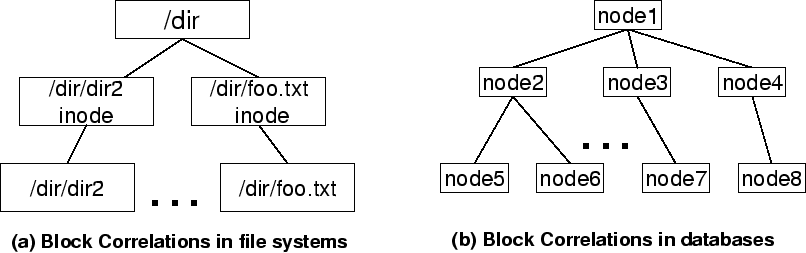
\includegraphics[width=\textwidth]{block_correlations}
\caption{数据块关联性的例子}
\label{fig:block_correlations}
\end{figure}
数据块关联性(Block Correlations)广泛存在于存储系统中。如图\ref{fig:block_correlations}所示,两个或以上的数据块存在语义关系时,它们便是相互关联的。如图中的目录块“/dir”与inode块“/dir/foo.txt”直接关联,后者与其对应的文件块直接关联。在这种情况下,目录块“/dir”与“/dir/foo.txt”的文件块间接关联。

需要指出的是,块关联性是静态存在的,与工作负载的运行过程无关,在文件系统结构不发生变化的情况下,这种静态关联能够长时间保持。另一方面,这种静态的关联通常会在工作负载动态访问数据的过程中得到体现,即,多数应用在访问数据块时会遵循块关联关系依次访问。因此,挖掘数据块关联对分析应用访问模式,数据缓存策略以及数据分布策略等技术能够提供极大帮助。

Zhenmin Li等人\cite{c_miner}于2004年提出了用于块数据关联性挖掘的C-Miner算法,该算法衍生于数据挖掘领域中的频繁序列挖掘算法(Frequent Sequence Mining)。
频繁序列挖掘是一种在序列数据库中发现频繁子序列的关联分析方法。当子序列出现在序列数据库中至少指定数目的序列(min support)中时,被认为是频繁的。例如,数据块访问序列数据库具有五个序列:
\begin{equation*}
    D = \{ abced, abcef, abijc, aklc \}
\end{equation*}
若取最小支持数为4,那么该数据库就包括以下频繁序列$\{ ab:4, ac:5, bc:4 ,abc:4 \}$。因此可以说,以上频繁序列中的文件具有关联。

C-Minier算法对传统的频繁序列挖掘算法进行改进,降低了计算复杂度,在性能方面针对文件系统的特有结构进行了优化,该算法在文件预取、数据分布调度等研究领域取得了不同程度的应用。

例如Jianwei Liao等
\cite{Prefetching_on_storage_servers_through_mining_access_patterns_on_blocks}
在存储服务器端应用C-Miner算法挖掘数据块关联,同时将客户端的应用信息嵌入到I/O访问请求中共同传递到服务端,两者结合以提升文件预取性能。Zhang等人\cite{composite_file}设计实现了一种聚合文件系统,其核心技术是将经常连续访问,具有较高关联度的小文件聚合组织成一个大文件,并用新的inode作为这个大文件的索引,在访问其中小文件的同时将聚合的其他小文件一并取出,从而大幅提升小文件访问性能。

然而频繁序列挖掘算法存在一定的缺陷,对于较长的访问序列,频繁子序列挖掘的计算代价太高。
\subsubsection*{N-gram模型}
N-gram模型是自然语言处理中一种基于统计方法的语言模型。其基本思想是在处理文本序列时,定义一个大小为$n$的上下文滑动窗口,每个窗口内截取的文本片段就成为gram。在此基础上,对所有gram出现的次数进行统计,并且按照预设的阈值进行过滤,最后形成gram列表。该模型基于这样的假设:第n个词的出现只与前n-1个词相关,而与其他任何词都无关(即n-1阶马尔科夫性质),整句的概率就是各个词出现概率的乘积。

事实上,N-gram模型与上文提到的频繁序列挖掘具有相似之处,gram相当于频繁子序列,形成gram的阈值相当于最小支持数。区别在于,gram的形成必须是严格相邻的n个元素,而频繁子序列没有这一要求。

Subedi等人\cite{stacker}
在Calibrun超算和Titan Cray XK7平台上,基于DataSpace框架\cite{dataspace}
基础上设计实现了一个名为“Stacker”的分层存储管理框架。
\begin{figure}[htp]
\centering
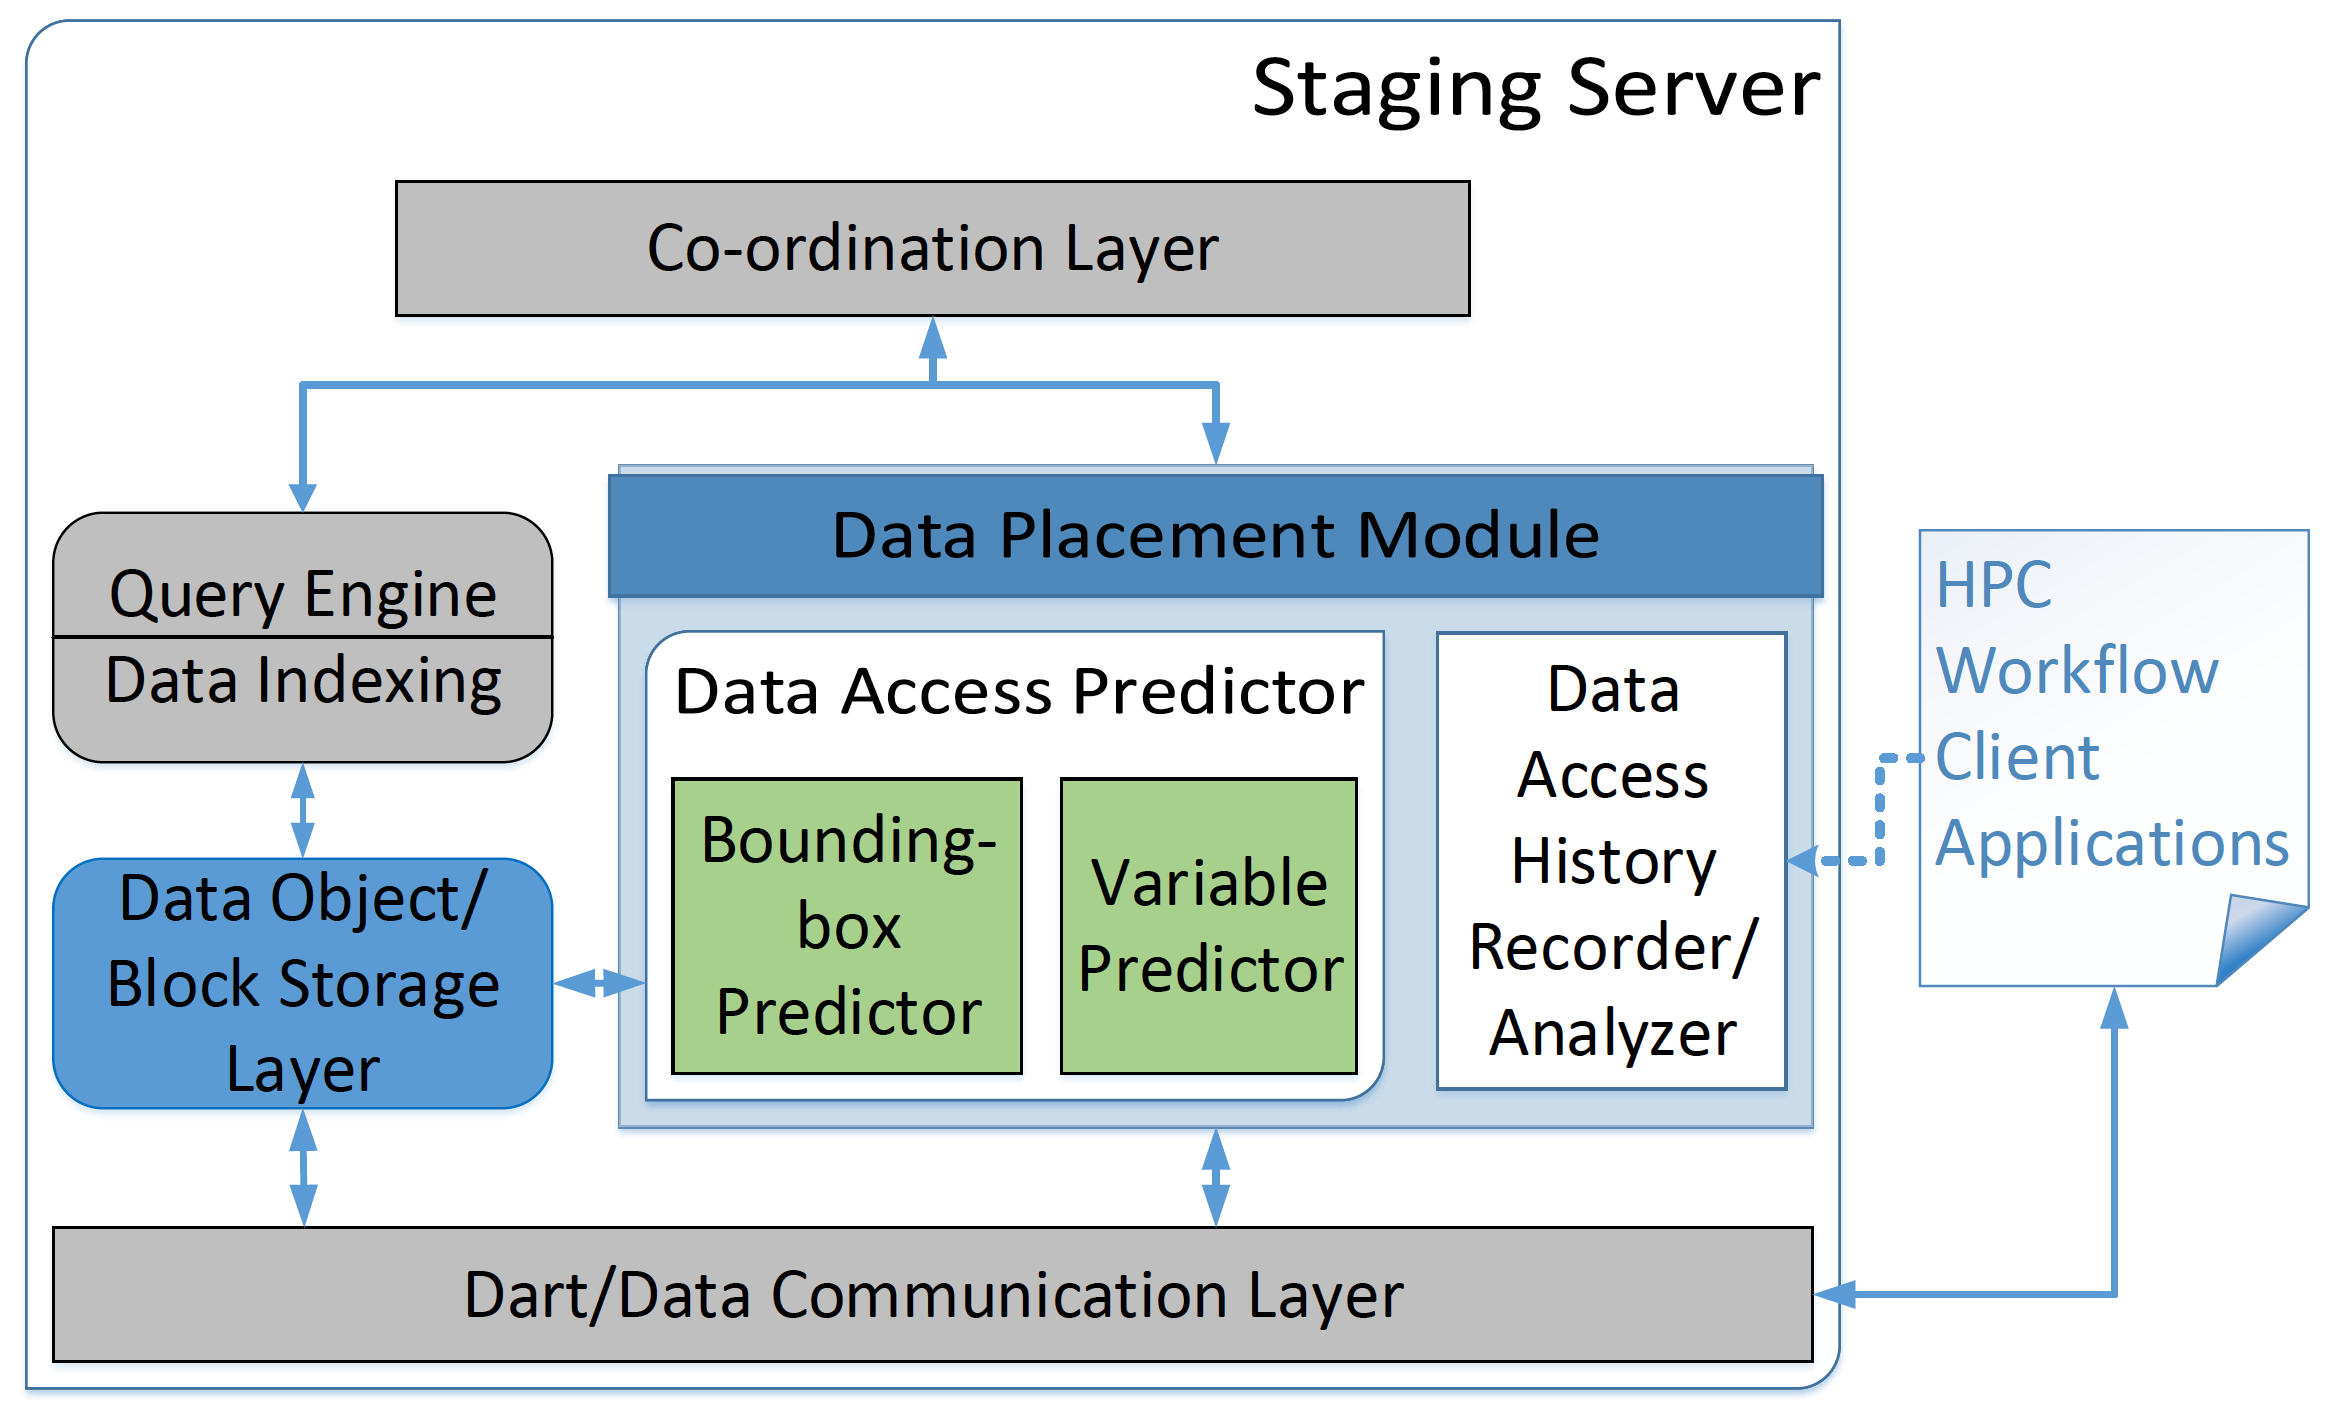
\includegraphics[width=\textwidth]{stacker}
\caption{多层存储管理框架Stacker的架构}
\label{fig:stacker}
\end{figure}

Stacker主要面向的工作负载是XGC1\cite{XGC1},S3D\cite{S3D}等数据量可达100PB级的模拟仿真计算。仿真结果可视化是这类负载的重要组成部分,过大规模的数据无法完全存放于共享内存中,需要SSD阵列及磁盘阵列组成多级存储,同时为了满足可视化应用需求,数据从SSD预取到内存必须及时、准确,因此数据迁移管理是该存储系统中的技术难点。Stacker的设计目的是通过机器学习的方法捕捉应用的数据访问模式,并利用访问模式的特征指导数据迁移模块进行高效的数据预取和下载。与此同时,在如此复杂的应用背景下,仅仅考虑单应用的访问模式是远远不够的,必须考虑到大规模并行计算应用背景下,多个不同任务进程之间表现的不同的I/O行为和干扰。为此,Stacker针对此类科学计算应用负载进行了优化,采用N-gram模型对应用的访问模式进行识别和预测。预测的主要内容包括访问的变量名,以及变量内部的偏移和大小。

以变量名访问模式为例,当存储服务器收到一个新的读数据请求,Stacker模块将会对此前的n条访问历史进行分析,提取其中的1-gram到n-gram序列并更新gram列表中。与此同时,分别进行n-gram,n-1-gram直至2-gram的查找匹配,最终将列表中出现频率最高的匹配结果作为该时刻之后变量名访问的预测。

N-gram模型的劣势与C-Miner算法类似,随着分析的序列长度增加,匹配的时间复杂度和gram列表存储的空间复杂度会迅速增加,Stacker的设计中gram的长度通常不超过20。因此比较适用于大文件的对象存储,小文件访问性能未能证明其有效性。




\section{本文主要工作}
本文的主要研究目标是分层存储系统中的热点数据识别,通过一系列理论研究和实践,基于文件系统与自然语言处理隐含的相似性建立了词嵌入模型与循环神经网络模型,将热点数据识别问题转化为冷热数据二分类问题展开研究。

目前分层存储管理优化方式主要包括两方面:一是挖掘文件的关联性(Block Correlation),二是动态追踪应用的I/O行为并加以分析,实现I/O行为预测(热数据识别),以指导数据迁移模块进行主动的数据预取和缓存替换。以往的研究具有局限性,例如,对文件的关联性挖掘局限于目录树结构表现出的文件关系,没有对文件或目录命名隐含的语义关系予以分析;I/O行为的分析通常只针对短期内的访问规律,没有在长时间跨度上进行分析。为解决上述问题,探索新的分层管理优化方式,本文做了以下几方面的工作:

1)文件的向量化表示。数据块关联(Block Correlation)在文件系统中广泛存在,且这种数据间的联 系通常比较稳定,在目录结构不发生变化的情况下,一般不受工作负载的运行状 态影响。反过来,工作负载访问文件的部分规律是由文件之间的固有关系决定的。 如果能显示地挖掘出文件之间的联系,可以为存储系统的数据分布策略、迁移策 略等提供帮助。本文从文件之间语义关系入手,建立了词嵌入模型将文件和目录映射为向量,将文件之间的关联分析转化为向量运算。

2)基于循环神经网络的文件分类模型。本文对冷热文件分类任务进行了形式化定义,在文件向量化表示的基础上,建立了GRU循环神经网络对应用的I/O序列进行分析和文件分类。

3)在上述两项工作的基础上,本文在GlusterFS架构的基础上设计了一套分层存储管理框架,该框架对Tiering模块、CTR模块以及GFDB数据库等进行了改进设计,将文件向量作为额外的元数据,并将循环神经网络嵌入到CTR模块中代替传统的LRU缓存算法指导数据迁移。





4)以开源工程编译任务作为工作负载,设计相关实验对上述两项模型进行验证。


\section{论文结构}
本文共包含六个章节,其结构组织编排如下:

第一章绪论,对当前分层存储系统在计算机领域的广泛应用进行了阐述,尤其是伴随着NVMe、SSD等高性能存储介质相关技术的飞速发展,分层存储管理中的热数据识别和数据迁移技术成为分层存储管理优化的关键。本章对相关领域发展概况进行了介绍,重点描述和分析了几项主动预取技术,作为本课题研究的引子。

第二章为相关背景工作介绍。本章在第一节陈述了分层存储模型的定义,并对当前主流的4层存储模型进行了阐述。与4层存储模型相对应的是数据的分类方式,主要包括I/O密集型、任务关联型、重要与敏感数据、归档数据等。在此存储模型下,数据分类的指标可归结为I/O性能要求、任务关联性以及外部环境要求等三方面。本文的研究针对任务关联性指标展开,目的是为了捕捉文件之间的静态关联和较长时间跨度的任务关联性。第二节对自然语言处理领域的两个重要内容进行了介绍,一是词嵌入技术的发展概况和基本原理,尤其是近年来广泛应用的Word2Vec模型。随后,介绍了循环神经网络的基本概况,阐明其在自然语言处理和序列处理中的广泛应用。

第四章是本课题的理论模型部分,内容包括基于词嵌入模型的文件关联分析和基于循环神经网络的文件分类模型。在文件关联分析部分,本文实现了文件的向量化表示,将文件之间的关联分析转化为向量运算。在基于循环神经网络的文件分类模型中,本文对冷热文件分类任务进行了形式化定义,在文件向量化表示的基础上,建立了GRU循环神经网络对应用的I/O序列进行分析和文件分类。


第五章以第四章内容为理论基础,在GlusterFS架构的基础上设计了一套分层存储管理框架,该框架对Tiering模块、CTR模块以及GFDB数据库等进行了改进设计,将文件向量作为额外的元数据,并将循环神经网络嵌入到CTR模块中代替传统的LRU缓存算法指导数据迁移。

第六章为实验部分。在实验涉及的工作负载选取上,充分考虑了开源工程编译任务的特点,将其列为模型验证初期实验的首选,设计了实验数据采集方案和具体的实验实施方案,给出了相应的评估标准,最后就实验结果进行了分析。